\section{Stabilität -- Nyquistkriterium}{126}
\label{offener Regelkreis}

Die Stabilität eines Regelkreises kann mit dem Nyquistkriterium viel einfacher betrachtet werden. 
Dafür wird der \textbf{Frequenzgang} $\bm{G_0(\jimg \omega)}$ \textbf{des offenen Regelkreises} betrachtet.

Ausserdem gibt das Nyquistkriterium an, wie robust ein Regelkreis ist.

\begin{minipage}[c]{0.48\columnwidth}
    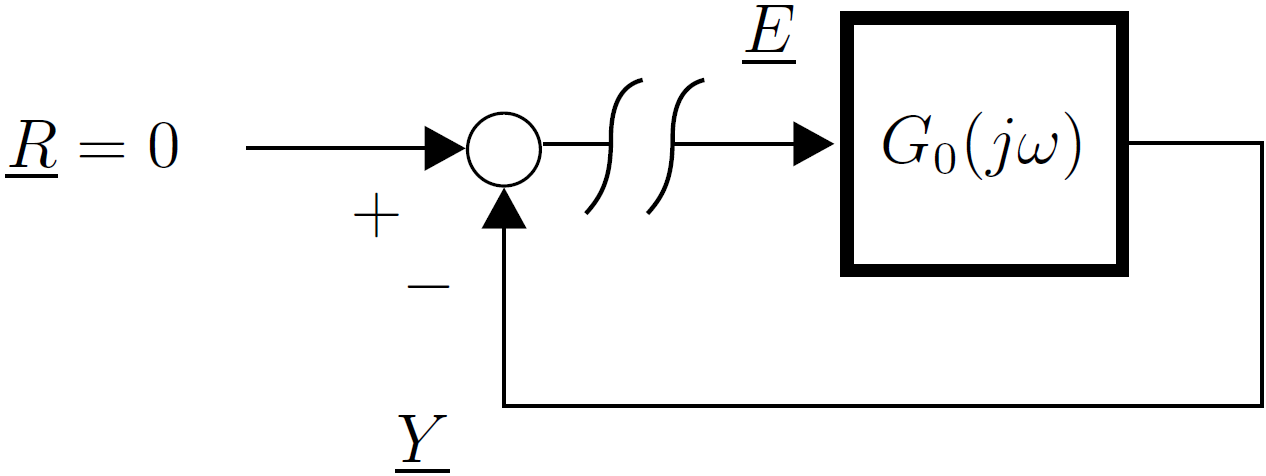
\includegraphics[width=\columnwidth]{images/offener_regelkreis.png}
\end{minipage}
\hfill
\begin{minipage}[c]{0.48\columnwidth}
    \begin{center}
        Frequenzgang des offenen Regelkreises
    \end{center}
    $$ \boxed{ G_0(\jimg \omega) = \frac{\underline{Y}}{\underline{E}} } $$
\end{minipage}



\example{Kreisschaltung mit mehreren Blöcken}
\label{Kreisschaltung mehrere Bloecke}

Folgendes System besitzt ein Eingangssignal $\underline{R}$ und vier Ausgangssignale $\underline{Y}$\\
Es sollen der Frequenzgang des offenen Regelkreises $G_0(\jimg \omega)$, sowie ausgewählte UTFs des Systems beschrieben werden.

$$ G_0(\jimg \omega) = G_1(\jimg \omega) \cdot G_2(\jimg \omega) \cdot G_3(\jimg \omega)  $$

\begin{minipage}[c]{0.5\columnwidth}
    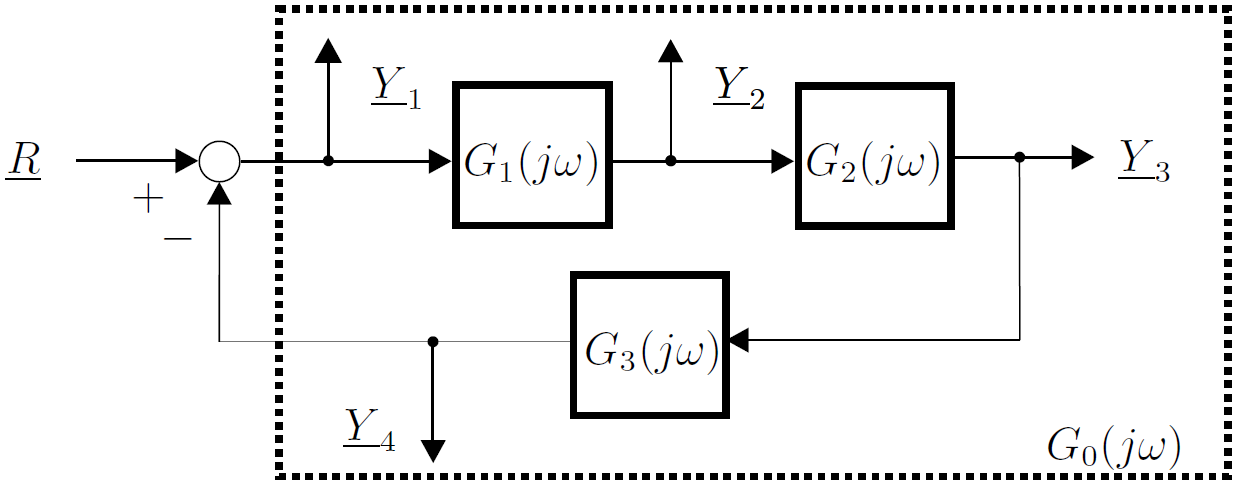
\includegraphics[width=\columnwidth]{images/kreisschaltung_mehrere_bloecke.png}
\end{minipage}
\hfill
\begin{minipage}[c]{0.48\columnwidth}
    $$ \frac{\underline{Y}_1}{\underline{R}} = \frac{1}{1 + G_1(\jimg \omega) \cdot G_2(\jimg \omega) \cdot G_3(\jimg \omega)} $$
    % $$ \frac{\underline{Y}_1}{\underline{R}} = \frac{G_1(\jimg \omega)}{1 + G_1(\jimg \omega) \cdot G_2(\jimg \omega) \cdot G_3(\jimg \omega)} $$
    $$ \frac{\underline{Y}_3}{\underline{R}} = \frac{G_1(\jimg \omega) \cdot G_2(\jimg \omega)}{1 + G_1(\jimg \omega) \cdot G_2(\jimg \omega) \cdot G_3(\jimg \omega)} $$
    % $$ \frac{\underline{Y}_4}{\underline{R}} = \frac{G_1(\jimg \omega) \cdot G_2(\jimg \omega) \cdot G_3(\jimg \omega)}{1 + G_1(\jimg \omega) \cdot G_2(\jimg \omega) \cdot G_3(\jimg \omega)} $$
\end{minipage}

\vspace{0.2cm}
\textbf{Hinweis:} Die Stabilität des Systems ist \textbf{unabhängig von der Reihenfolge der Teilsysteme} $G_{i}(\jimg \omega)$,
da die Stabilität durch den Nenner (bzw. die Polstellen) beschrieben wird.


\subsection{Stabilität im Nyquist-Diagramm}

Gedankenexperiment: Ein offener Regelkreis mit $G_0(\jimg \omega)$ (gemäss Abschnitt~\ref{offener Regelkreis}) wird um eine 
veränderbare Verstärkung $K$ ergänzt.


\subsubsection{Stabilität}

Wähle $K = K_0$, sodass sich die Ortskurve immer innerhalb des Einheitskreises befindet.
\vspace{0.1cm}
\begin{itemize}
    \item Befindet sich die Ortskurve eines Systems immer \textbf{innerhalb des Einheitskreises}, so ist der offene Regelkreis stabil. \\
        \textrightarrow\ Daraus folgt, dass auch der geschlossene Regelkreis stabil sein muss.
    \item Führungsübertragungsfunktion für $K \ll K_0$:\\
    $G_f(\jimg \omega) = \frac{K \cdot G_0(\jimg \omega)}{1 + K \cdot G_0(\jimg \omega)} \approx K \cdot G_0(\jimg \omega)$ 
\end{itemize}


\subsubsection{Grenzstabilität}

Wähle $K = K_{\rm krit} > K_0$, sodass die Ortskurve den Punkt $-1$ schneidet.
\vspace{0.1cm}
\begin{itemize}
    \item Ortskurve des offenen Regelkreises $G_0(\jimg \omega)$ verläuft \textbf{durch den Punkt $\boldsymbol{-1}$}, 
    \item Die Frequenz $\omega_{\pi}$, für die $G_0(\jimg \omega_{\pi})= -1 = \e^{- \pi}$ heisst \textbf{kritische Frequenz}. Mit dieser 
        kritischen Frequenz schwingt das System.
    \item Die Führungsübertragungsfunktion $G_f(\jimg \omega) = \frac { K \cdot G_0(\jimg \omega)}{1 + K \cdot G_0(\jimg \omega)}$ wird bei 
    der kritischen Frequenz zu $G_f(\jimg \omega_{\pi}) = \frac{-1}{1-1} = - \infty $ \textrightarrow\ Grenzstabilität
\end{itemize}


\subsubsection{Instabilität}

Wähle $K > K_{\rm krit}$
\vspace{0.1cm}
\begin{itemize}
    \item Ortskurve verläuft nicht mehr durch den Punkt $-1$
    \item Das System ist instabil
\end{itemize}


\subsection{Vereinfachtes Nyquistkriterium}{127-128}

Idee: Informationen über den \textbf{offenen Regelkreis} verwenden, um die \textbf{Stabillität des geschlossenen Regelkreises} 
zu beurteilen


\subsubsection{Vereinfachtes Nyquistkriterium}

\fbox{\parbox{0.95\columnwidth}{
\begin{itemize}
    \item Gemäss Abschnitt ~\ref{Kreisschaltung mehrere Bloecke}  wird $G_0 = \prod_i G_i$ gebildet aus den seriegeschalteten
        Teilsystemen des offenen Regelkreises \cbl{(\textrightarrow\ Produkt aller $G_i$ \textbf{im Feedback-Loop})}
    \item $G_0$ muss dabei einem \textbf{Prozess mit Ausgleich \cbl{(stabilen Prozess)}} entsprechen; zusätzlich 
    \textbf{dürfen} noch einer oder zwei Integratoren seriegeschaltet sein\\
        Mit Polen formuliert: Bei $G_0$ sind maximal zwei Pole bei Null erlaubt; alle weiteren Pole müssen in der linken Halbebene liegen
    \item Damit der geschlossene Regelkreis stabil ist, muss der kritische Punkt $-1$ \textbf{links} der Nyquistkurve von $G_0$ liegen,
        wenn diese in Richtung zunehmender Frequenz durchlaufen wird ($\omega = 0 \ldots \infty$) 
        \cbl{\textrightarrow\ 'links der Kurve': Man befindet sich \textbf{auf der Kurve} und 'schaut' nach links und muss
        den Punkt $-1$ 'sehen'}
\end{itemize}
}}


\example{Ortskurven stabiler Systeme}{128}

\textbf{Achtung:} Damit die Stabilität der gezeigten Systeme beurteilt werden kann, muss sichergestellt werden, dass auch die ersten
beiden Punkte des vereinfachten Nyquistkriteriums eingehalten werden!

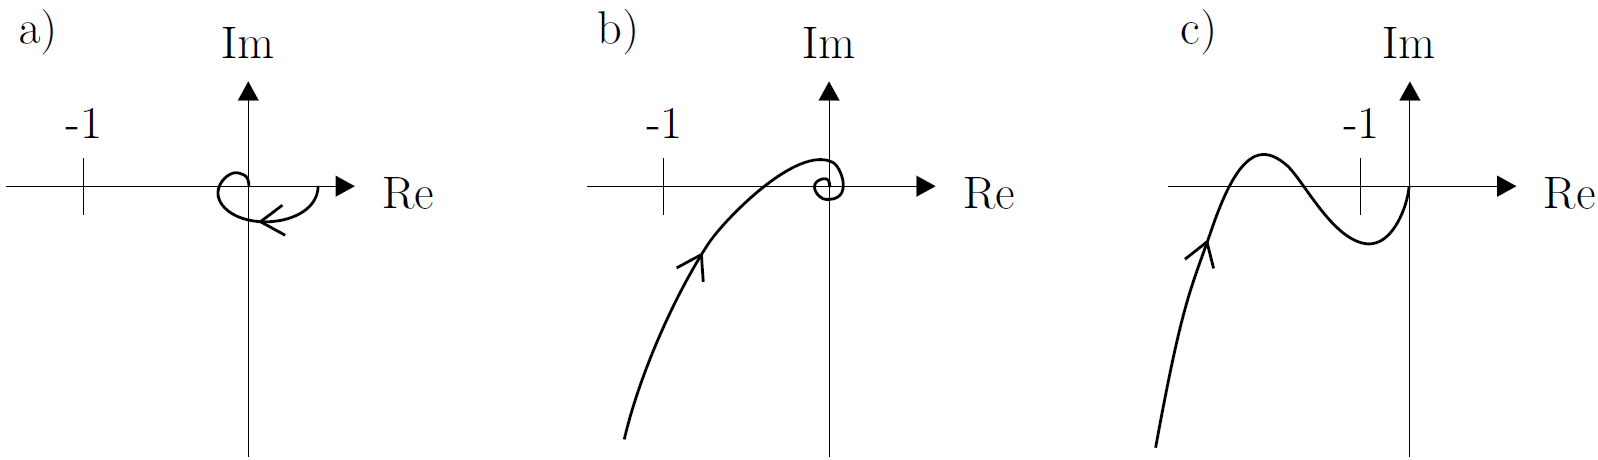
\includegraphics[width=\columnwidth]{images/nyquist_stabile_kurven.png}


\subsection{Stabilitätsreserven}

Wir möchten nicht nur Stabilität, sondern auch eine gewisse Stabilitätsreserve, um z.B. auch bei einem ungenau
modellierten Prozess oder einer sich ändernden Regelstrecke noch einen stabilen Regelkreis zu gewährleisten. 
\vspace{0.2cm}
\begin{outline}
    \1 \textbf{Auch ein stabiler Regelkreis kann sehr lange (ein)schwingen}
    \1 Stabilität / Grenzstabilität / Instabilität sind defnierte Bereiche
        \2 Es gibt nicht 'ein wenig stabil', 'ziemlich stabil', 'stabiler als...', 'instabiler als'
    \1 Allenfalls: Ein Regelkreis ist stabiler als ein anderer. Gemeint ist:
        \2 Ein Regelkreis ist besser gedämpft / schneller (eingeschwungen)
        \2 Ein Regelkreis ist robust -- er ist trotz gewissen Widerigkeiten im Regelkreis
        \2 \textbf{Ein Regelkreis bleibt stabil, auch wenn die Regelstrecke leicht ändert}
\end{outline}


\subsection{Stabilitätsreserven im Nyquistdiagramm}{129}


\begin{minipage}[c]{0.48\columnwidth}
    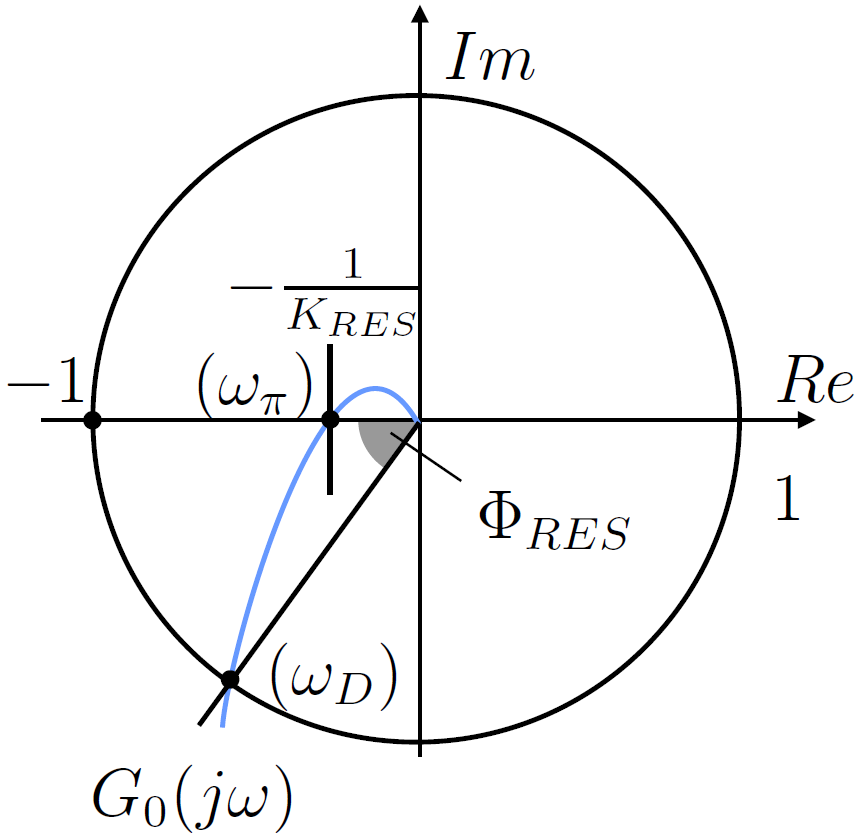
\includegraphics[width=\columnwidth]{images/stabilitaetsreserven_1.png}
\end{minipage}
\hfill
\begin{minipage}[c]{0.5\columnwidth}

    $$ \boxed{\Phi_{\rm RES} = \arctan \left( \frac{\Re{G_{0}(\jimg \omega_{D})}}{\Im{G_{0}(\jimg \omega_{D})}} \right) } $$
    $$ \boxed{\frac{1}{K_{\rm RES}} = \big| G_{0}(\jimg \omega_{\pi}) \big| } $$


     Ein System ist \textbf{stabil}, wenn eine der folgenden Bedingungen erfüllt ist:
     \vspace{0.2cm}

     \begin{itemize}
        \setlength\itemsep{4pt}
        \item $\omega_{\pi} > \omega_{D}$
        \item $G_{0}(\jimg \omega_{D}) = \e^{- \jimg \varphi}$ \quad mit $0 < \varphi < \pi$
        \item $0 > G_{0}(\jimg \omega_{\pi}) > -1 $
     \end{itemize}
\end{minipage}

\vspace{0.2cm}

\begin{itemize}
    \item Durchtrittsfrequenz $\omega_{D}$ \\
        Frequenz, bei der die Kurve den Einheitskreis durchquert: $| G_{0}(\jimg \omega_{D})| = 1 $ \\
        \textrightarrow\ Phasenreserve $\Phi_{\rm RES}$
    
    \item Phasenschnittfrequenz $\omega_{\pi}$ \\
        Frequenz, bei der die Kurve die reelle Achse durchquert: $\Im{G_{0}(\jimg \omega_{\pi})} = 0$\\
        \textrightarrow\ Verstärkungsreserve $K_{\rm RES}$
\end{itemize}


\subsubsection{Verstärkungsreserve $K_{\rm RES}$}

Die Verstärkungsreserve $K_{\rm RES}$ liefert direkt den Toleranzwert für den Fall, dass die \textbf{Modellunsicherheit} des 
offenen Regelkreises bei der \textbf{Verstärkung} liegt. \\
Der Abstand zur Ursprung bei der Phasenschnittfrequenz $\omega_{\pi}$ entspricht $\frac{1}{K_{\rm RES}}$ \\
\textrightarrow\ Wenn anstatt dem Nominalfrequenzgang $G_0(\jimg \omega)$ tatsächlich $K_{\rm RES} \cdot G_0(\jimg \omega)$ vorliegt, wird der
Regelkreis \textbf{grenzstabil}!


\subsubsection{Phasenreserve $\Phi_{\rm RES}$}

Die Phasenreserve $\Phi_{\rm RES}$ liefert einen Toleranzwert für den Fall, dass die \\
\textbf{Modellunsicherheit} des offenen Regelkreises bei der \textbf{Totzeit} liegt.

\textrightarrow\ Wenn anstatt dem Nominalfrequenzgang $G_0(\jimg \omega)$ tatsächlich $G_0(\jimg \omega) \cdot \e^{- \jimg \omega T_t}$ vorliegt, 
wird der Regelkreis \textbf{grenzstabil}!
\bigskip

Der Zusammenhang zwischen Phasendrehung und Totzeit ist
$$ \boxed{ T_t = \frac{\Phi_{\rm RES}}{\omega_D}  \quad \text{ wobei } [\Phi_{\rm RES}] = \rad } $$


\example{Einfluss von Stabilitätsreserven auf Nyquistdiagramm}

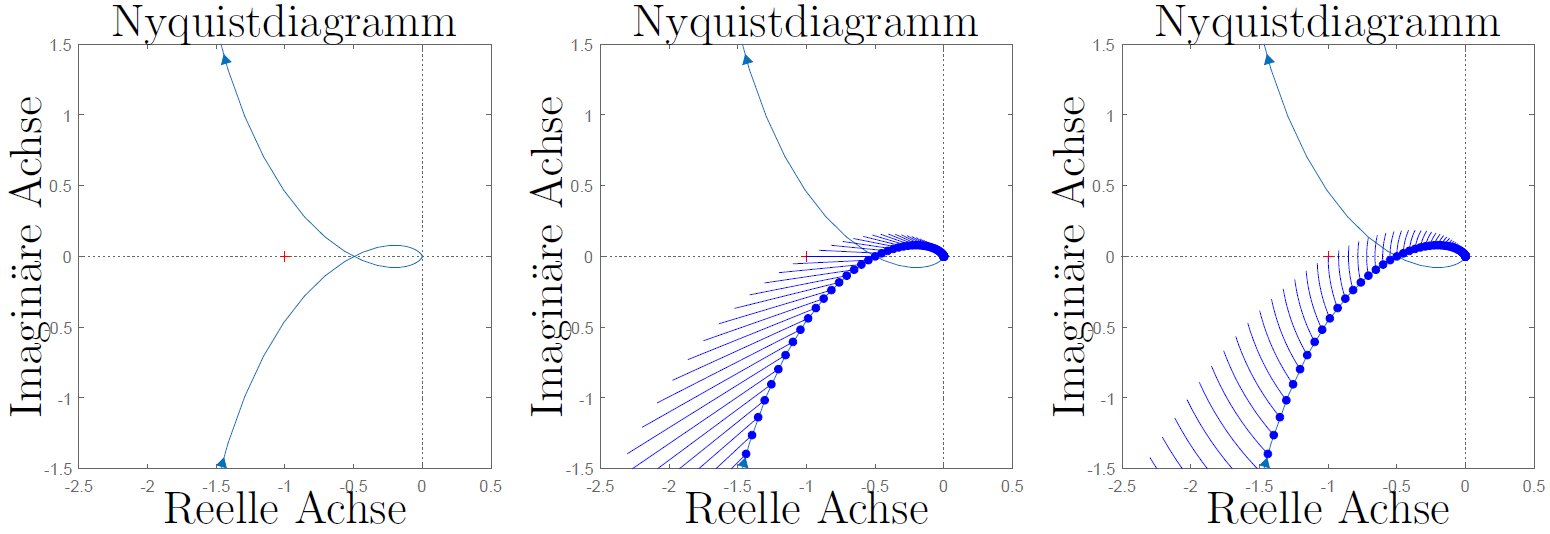
\includegraphics[width=\columnwidth]{images/nyquist_stabilitaetsreserven.png}

\begin{tabular}{ll}
    Mitte:  & Verstärkungsreserve streckt Kurve vom Ursprung aus \\
    Rechts: & Phasenreserve dreht jeden Punkt der Kurve um verschiedene Winkel $\omega \cdot T_t$ \\
            & um den Ursprung  
\end{tabular}


\subsubsection{Faustregeln für Reserven}{131}

\textbf{Hinweis:} Es besteht eine Kopplung zwischen den beiden Effekten!

\begin{itemize}
    \item Phasenreserve von $\Phi_{\rm RES} = 40 \degree \ldots 70 \degree$
    \item Verstärkungsreserve von $K_{\rm RES} > 4 \, (\approx 12 \, \deci \bel)$
\end{itemize}


\subsection{Nyquistdiagramme mit MatLab}

\lstinputlisting{snippets/nyquist.m}


\subsection{Vorgehen: Nyquistdiagramme zeichnen}

\begin{itemize}
    \item Werte für $G(\omega = 0)$ und $G(\omega = \infty)$ berechnen
    \item Anzahl $\jimg$ im Zähler \textbf{plus} Anzahl $\jimg$ im Nenner entspricht Anzahl Quadranten, welche zwischen $\omega = 0$ und 
        $\omega = \infty$ durchlaufen werden
    \item Pollstellen: $|G(\jimg \omega)|$ \textdownarrow\ ; $\angle G(\jimg \omega)$ \textdownarrow\ \textrightarrow\ Bewegung im Uhrzeigersinn
        \textrightarrow\ Bei den Nullstellen ist $\angle G(\jimg \omega) = \pm 45 \, \degree$
    \item Nullstellen: $|G(\jimg \omega)|$ \textuparrow\ ; $\angle G(\jimg \omega)$ \textuparrow\ ; \textrightarrow\ Bewegung im Gegenuhrzeigersinn
    \item Frequenzen der Pol- bzw. Nullstellen berechnen
\end{itemize}

